\documentclass[twoside]{article}
\usepackage[accepted]{aistats2021}

\special{papersize = 8.5in, 11in}
\setlength{\pdfpageheight}{11in}
\setlength{\pdfpagewidth}{8.5in}

\usepackage{amsmath, amsfonts, amsthm, amssymb}
\usepackage{graphicx}
\usepackage{hyperref}
\hypersetup{
	colorlinks=true,
	linkcolor=blue,
	citecolor=blue
}
\usepackage[parfill]{parskip}
\usepackage{algpseudocode}
\usepackage{algorithm}
\usepackage{enumerate}
\usepackage[shortlabels]{enumitem}
\usepackage{mathtools}
\usepackage{tikz}
\usepackage{verbatim}
\usepackage{microtype}
\usepackage{bm}

\usepackage{natbib}
\renewcommand{\bibname}{REFERENCES}
\renewcommand{\bibsection}{\subsubsection*{\bibname}}

\DeclareFontFamily{U}{mathx}{\hyphenchar\font45}
\DeclareFontShape{U}{mathx}{m}{n}{<-> mathx10}{}
\DeclareSymbolFont{mathx}{U}{mathx}{m}{n}
\DeclareMathAccent{\wb}{0}{mathx}{"73}

\DeclarePairedDelimiterX{\norm}[1]{\lVert}{\rVert}{#1}
\DeclarePairedDelimiterX{\seminorm}[1]{\lvert}{\rvert}{#1}

% Make a widecheck symbol (thanks, Stack Exchange!)
\DeclareFontFamily{U}{mathx}{\hyphenchar\font45}
\DeclareFontShape{U}{mathx}{m}{n}{
	<5> <6> <7> <8> <9> <10>
	<10.95> <12> <14.4> <17.28> <20.74> <24.88>
	mathx10
}{}
\DeclareSymbolFont{mathx}{U}{mathx}{m}{n}
\DeclareFontSubstitution{U}{mathx}{m}{n}
\DeclareMathAccent{\widecheck}{0}{mathx}{"71}
% widecheck made

\newcommand{\eqdist}{\ensuremath{\stackrel{d}{=}}}
\newcommand{\Graph}{\mathcal{G}}
\newcommand{\Reals}{\mathbb{R}}
\newcommand{\iid}{\overset{\text{i.i.d}}{\sim}}
\newcommand{\convprob}{\overset{p}{\to}}
\newcommand{\convdist}{\overset{w}{\to}}
\newcommand{\Expect}[1]{\mathbb{E}\left[ #1 \right]}
\newcommand{\Risk}[2][P]{\mathcal{R}_{#1}\left[ #2 \right]}
\newcommand{\Prob}[1]{\mathbb{P}\left( #1 \right)}
\newcommand{\iset}{\mathbf{i}}
\newcommand{\jset}{\mathbf{j}}
\newcommand{\myexp}[1]{\exp \{ #1 \}}
\newcommand{\abs}[1]{\left \lvert #1 \right \rvert}
\newcommand{\restr}[2]{\ensuremath{\left.#1\right|_{#2}}}
\newcommand{\ext}[1]{\widetilde{#1}}
\newcommand{\set}[1]{\left\{#1\right\}}
\newcommand{\seq}[1]{\set{#1}_{n \in \N}}
\newcommand{\floor}[1]{\left\lfloor #1 \right\rfloor}
\newcommand{\Var}{\mathrm{Var}}
\newcommand{\Cov}{\mathrm{Cov}}
\newcommand{\diam}{\mathrm{diam}}

\newcommand{\emC}{C_n}
\newcommand{\emCpr}{C'_n}
\newcommand{\emCthick}{C^{\sigma}_n}
\newcommand{\emCprthick}{C'^{\sigma}_n}
\newcommand{\emS}{S^{\sigma}_n}
\newcommand{\estC}{\widehat{C}_n}
\newcommand{\hC}{\hat{C^{\sigma}_n}}
\newcommand{\vol}{\text{vol}}
\newcommand{\spansp}{\mathrm{span}~}
\newcommand{\1}{\mathbf{1}}

\newcommand{\Linv}{L^{\dagger}}
\DeclareMathOperator*{\argmin}{argmin}
\DeclareMathOperator*{\argmax}{argmax}
\DeclareMathOperator*{\esssup}{ess\,sup}

\newcommand{\emF}{\mathbb{F}_n}
\newcommand{\emG}{\mathbb{G}_n}
\newcommand{\emP}{\mathbb{P}_n}
\newcommand{\F}{\mathcal{F}}
\newcommand{\D}{\mathcal{D}}
\newcommand{\R}{\mathcal{R}}
\newcommand{\Rd}{\Reals^d}
\newcommand{\Nbb}{\mathbb{N}}

%%% Vectors
\newcommand{\thetast}{\theta^{\star}}
\newcommand{\betap}{\beta^{(p)}}
\newcommand{\betaq}{\beta^{(q)}}
\newcommand{\vardeltapq}{\varDelta^{(p,q)}}
\newcommand{\lambdavec}{\boldsymbol{\lambda}}

%%% Matrices
\newcommand{\X}{X} % no bold
\newcommand{\Y}{Y} % no bold
\newcommand{\Z}{Z} % no bold
\newcommand{\Lgrid}{L_{\grid}}
\newcommand{\Dgrid}{D_{\grid}}
\newcommand{\Linvgrid}{L_{\grid}^{\dagger}}
\newcommand{\Lap}{L}
\newcommand{\NLap}{{\bf N}}
\newcommand{\PLap}{{\bf P}}
\newcommand{\Id}{I}

%%% Sets and classes
\newcommand{\Xset}{\mathcal{X}}
\newcommand{\Vset}{\mathcal{V}}
\newcommand{\Sset}{\mathcal{S}}
\newcommand{\Hclass}{\mathcal{H}}
\newcommand{\Pclass}{\mathcal{P}}
\newcommand{\Leb}{L}
\newcommand{\mc}[1]{\mathcal{#1}}

%%% Distributions and related quantities
\newcommand{\Pbb}{\mathbb{P}}
\newcommand{\Ebb}{\mathbb{E}}
\newcommand{\Qbb}{\mathbb{Q}}
\newcommand{\Ibb}{\mathbb{I}}

%%% Operators
\newcommand{\Tadj}{T^{\star}}
\newcommand{\dive}{\mathrm{div}}
\newcommand{\dif}{\mathop{}\!\mathrm{d}}
\newcommand{\gradient}{\mathcal{D}}
\newcommand{\Hessian}{\mathcal{D}^2}
\newcommand{\dotp}[2]{\langle #1, #2 \rangle}
\newcommand{\Dotp}[2]{\Bigl\langle #1, #2 \Bigr\rangle}

%%% Misc
\newcommand{\grid}{\mathrm{grid}}
\newcommand{\critr}{R_n}
\newcommand{\dx}{\,dx}
\newcommand{\dy}{\,dy}
\newcommand{\dr}{\,dr}
\newcommand{\dxpr}{\,dx'}
\newcommand{\dypr}{\,dy'}
\newcommand{\wt}[1]{\widetilde{#1}}
\newcommand{\wh}[1]{\widehat{#1}}
\newcommand{\ol}[1]{\overline{#1}}
\newcommand{\spec}{\mathrm{spec}}
\newcommand{\LE}{\mathrm{LE}}
\newcommand{\LS}{\mathrm{LS}}
\newcommand{\SM}{\mathrm{SM}}
\newcommand{\OS}{\mathrm{OS}}
\newcommand{\PLS}{\mathrm{PLS}}

%%% Order of magnitude
\newcommand{\soom}{\sim}

%%% Theorem environments
\newtheorem{theorem}{Theorem}
\newtheorem{conjecture}{Conjecture}
\newtheorem{lemma}{Lemma}
\newtheorem{example}{Example}
\newtheorem{corollary}{Corollary}
\newtheorem{proposition}{Proposition}
\newtheorem{assumption}{Assumption}
\newtheorem{remark}{Remark}

\theoremstyle{definition}
\newtheorem{definition}{Definition}[section]
\theoremstyle{remark}

\begin{document}
	
\runningtitle{Minimax Optimal Laplacian Smoothing}
	
\twocolumn[

	\aistatstitle{Minimax Optimal Regression over Sobolev Spaces via Laplacian Regularization on Neighborhood Graphs}
	
	\aistatsauthor{Alden Green \And Sivaraman Balakrishnan \And Ryan J. Tibshirani}

	\aistatsaddress{Carnegie Mellon University \And Carnegie Mellon University \And Carnegie Mellon University}]
	
\begin{abstract}
	In this paper we study the statistical properties of Laplacian smoothing, a graph-based approach to nonparametric regression. Under standard regularity conditions, we establish upper bounds on the error of the Laplacian smoothing estimator \smash{$\wh{f}$}, and a goodness-of-fit test also based on \smash{$\wh{f}$}. These upper bounds match the minimax optimal estimation and testing rates of convergence over the first-order Sobolev class $H^1(\Xset)$, for $\Xset \subseteq \Rd$ and $1 \leq d < 4$; in the estimation problem, for $d = 4$, they are optimal modulo a $\log n$ factor. Additionally, we prove that Laplacian smoothing is manifold-adaptive: if $\Xset \subseteq \R^d$ is an $m$-dimensional manifold with $m < d$, then the error rate of Laplacian smoothing (in either estimation or testing) depends only on $m$, in the same way it would if $\Xset$ were a full-dimensional set in $\Reals^m$.
\end{abstract}

\section{INTRODUCTION}

We adopt the standard setup in nonparametric regression, where we observe samples $(X_1,Y_1),\ldots,(X_n,Y_n)$ that are i.i.d.\ draws from the model 
\begin{equation}
\label{eqn:signal_plus_noise_model}
Y_i = f_0(X_i) + \varepsilon_i, \quad \epsilon_i \sim N(0,1), 
\end{equation}
where $\varepsilon_i$ is independent of $X_i$. Our goal is to perform statistical inference on the unknown regression function $f_0$, by which we mean either \emph{estimating} $f_0$ or more simply \emph{testing} whether $f_0 = 0$, i.e., whether there is any signal present. 

Laplacian smoothing \citep{smola2003} is a penalized least squares estimator, defined over a graph. Let $G = (V,W)$ be a weighted undirected graph with vertices $V=\{1,\ldots,n\}$, associated with $\{X_1,\ldots,X_n\}$, the Laplacian smoothing estimator \smash{$\wh{f}$} is given by
\begin{equation}
\label{eqn:laplacian_smoothing}
\wh{f} =  \argmin_{f \in \Reals^n} \; \sum_{i = 1}^{n}(Y_i - f_i)^2 + \rho \cdot f^\top \Lap f. 
\end{equation}
Here $\Lap$ is the graph Laplacian matrix (to be defined in Section~\ref{sec:problem_setup_and_background}), $G$ is typically a geometric graph (such as a $k$-nearest-neighbor or neighborhood graph), $\rho \geq 0$ is a tuning parameter, and the penalty
\begin{equation*}
f^\top \Lap f = \frac{1}{2} \sum_{i,j = 1}^{n} W_{ij}(f_i - f_j)^2
\end{equation*}
encourages \smash{$\wh{f}_i \approx \wh{f}_j$} when $X_i \approx X_j$. Assuming \eqref{eqn:laplacian_smoothing} is a reasonable estimator of $f_0$, the statistic
\begin{equation}
\label{eqn:laplacian_smoothing_test}
\wh{T} = \frac{1}{n} \| \wh{f} \|_2^2 
\end{equation}
would in turn be a reasonable way to test $f_0 = 0$. 

Of course there are many methods for nonparametric regression (see, e.g., \citet{gyorfi2006,wasserman2006,tsybakov2008_book}), but Laplacian smoothing has its own set of advantages. For instance:
\begin{itemize}
	\item \emph{Computational ease.} Laplacian smoothing is fast, easy, and stable to compute. The estimate \smash{$\wh{f}$} can be computed by solving a symmetric diagonally dominant linear system. There are by now various nearly-linear-time solvers for this problem (see e.g., the seminal papers of \citet{spielman2011,spielman2013,spielman2014}, or the overview by \citet{vishnoi2012} and references therein).
	\item \emph{Generality.} Laplacian smoothing is well-defined whenever one can associate a graph with observed responses. This generality lends itself to many different data modalities, e.g., text and image classification, as in \citet{kondor2002,belkin03a,belkin2006}.
	\item \emph{Weak supervision.} Although we study Laplacian smoothing in the supervised problem setting \eqref{eqn:signal_plus_noise_model}, the method can be adapted to the semi-supervised or unsupervised settings, as in \citet{zhu2003semisupervised,zhou2005learning,nadler09}. %,slepcev17,calder2019b,dunlop2020}.
\end{itemize}

For these reasons, a body of work has emerged that analyzes the statistical properties of Laplacian smoothing, and graph-based methods more generally. Roughly speaking, this work can be divided into two categories, based on the perspective they adopt. 
\begin{itemize}
	\item \emph{Fixed design perspective.} Here one treats the design points $X_1,\ldots,X_n$ and the graph $G$ as fixed, and carries out inference on $f_0(X_i)$, $i=1,\ldots,n$. In this problem setting, tight upper bounds have been derived on the error of various graph-based methods (e.g., \citet{wang2016,hutter2016,sadhanala16,sadhanala17,kirichenko2017,kirichenko2018}) and tests (e.g., \citet{sharpnack2010identifying,sharpnack2013b,sharpnack2013,sharpnack2015}), which certify that such procedures are \emph{optimal} over ``function'' classes (in parentheses because these classes really model the $n$-dimensional vector of evaluations). The upside of this work is its generality: in this setting $G$ need not be a geometric graph, but in principle it could be any graph over $V=\{1,\ldots,n\}$. The downside is that, in the context of nonparametric regression, it is as not natural to think of the evaluations of $f_0$ as exhibiting smoothness over some fixed pre-defined graph $G$, and more natural to speak of the smoothness of the function $f_0$ itself. 
	\item \emph{Random design perspective.} Here one treats the design points $X_1,\ldots,X_n$ as independent samples from some distribution $P$ supported on a domain $\Xset \subseteq \Rd$. Inference is drawn on the regression function $f_0: \Xset \to \Reals$, which is typically assumed to be smooth in some \emph{continuum} sense, e.g., it possesses a first derivative bounded in $L^{\infty}$ (H\"{o}lder) or $\Leb^2$ (Sobolev) norm. To conduct graph-based inference, the user first builds a neighborhood graph over the random design points---so that $W_{ij}$ is large when $X_i$ and $X_j$ are close in (say) Euclidean distance---and then computes e.g., \eqref{eqn:laplacian_smoothing} or \eqref{eqn:laplacian_smoothing_test}. In this context, various graph-based procedures have been shown to be \emph{consistent}: as $n \to \infty$, they converge to a continuum limit (see \citet{belkin07,vonluxburg2008,trillos2018} among others). However, until recently such statements were not accompanied by error rates, and even so, such error rates as have been proved \citep{lee2016,trillos2020} are not optimal over continuum function spaces, such as H\"{o}lder or Sobolev classes. 
\end{itemize}
The random design perspective bears a more natural connection with nonparametric regression (the focus in this paper), as it allows us to formulate smoothness based on $f_0$ itself (how it behaves as a continuum function, and not just its evaluations at the design points). In this paper, we will adopt the random design perspective, and seek to answer the following question:
\begin{quote}{When $f_0$ is assumed to smooth in a continuum sense, does Laplacian smoothing achieve optimal performance for estimation and goodness-of-fit testing?} 
\end{quote}
This is no small question---arguably, it is \emph{the} central question of nonparametric regression---and without an answer one cannot fully compare the statistical properties of Laplacian smoothing to alternative methods. It also seems difficult to answer: as we discuss next, there is a fundamental gap between the \emph{discrete} smoothness imposed by the penalty $f^\top \Lap f$ in problem \eqref{eqn:laplacian_smoothing} and the \emph{continuum} smoothness assumed on $f_0$, and in order to obtain sharp upper bounds we will need to bridge this gap in a suitable sense.

\section{SUMMARY OF RESULTS}

\paragraph{Advantages of the Discrete Approach.} 

In light of this last point, it is worth asking whether there is any \emph{statistical} advantage to solving a discrete problem such as \eqref{eqn:laplacian_smoothing} (setting aside computational considerations for the moment). After all, we could have instead solved the following variational problem:
\begin{equation}
\label{eqn:thin_plate_spline}
\wt{f} = \argmin_{f : \Xset \to \Reals} \; \sum_{i = 1}^{n} \bigl(Y_i - f(X_i)\bigr)^2 + \rho \hspace{-2pt} \int_{\Xset} \|\nabla f(x)\|_2^2 \,dx,
\end{equation}
where the optimization is performed over all functions for which the criterion is well-defined and finite (continuous functions $f$ that have a weak derivative $\nabla f$ in $L^2(\Xset)$). Analogously, for testing, we could use:
\begin{equation}
\label{eqn:thin_plate_spline_test}
\wt{T} = \| \wt{f} \|_n^2 = \frac{1}{n} \sum_{i=1}^n \wt{f}(X_i)^2.
\end{equation}
The penalty term in \eqref{eqn:thin_plate_spline} leverages the assumption that $f_0$ has a smooth derivative in a seemingly natural way. Indeed, the estimator \smash{$\wt{f}$} and statistic \smash{$\wt{T}$} are well-known: for $d = 1$, \smash{$\wt{f}$} is the familiar \emph{smoothing spline}, and for $d>1$, it is type of a \emph{thin-plate spline}. The statistical properties of smoothing and thin-plate splines are well-understood \citep{vandergeer2000,liu2019}. As we discuss later, the Laplacian smoothing problem \eqref{eqn:laplacian_smoothing} can be viewed as a discrete and noisy approximation to \eqref{eqn:thin_plate_spline}. At first blush, this suggests that Laplacian smoothing should at best inherit the statistical properties of \eqref{eqn:thin_plate_spline}, and at worst may have meaningfully larger error.

However, as we shall see the actual story is quite different: remarkably, Laplacian smoothing enjoys optimality properties even in settings where the thin-plate spline estimator \eqref{eqn:thin_plate_spline} is not well-posed (to be explained shortly); Tables~\ref{tbl:estimation_rates} and~\ref{tbl:testing_rates} summarize. As we establish in Theorems~\ref{thm:laplacian_smoothing_estimation1}-\ref{thm:laplacian_smoothing_testing_manifold}, when computed over an appropriately formed neighborhood graph, Laplacian smoothing estimators and tests are minimax optimal over first-order \emph{continuum} Sobolev balls. This holds true either when $\Xset \subseteq \Rd$ is a full-dimensional domain and $d = 1,2,$ or $3$, or when $\Xset$ is a manifold embedded in $\Rd$ of intrinsic dimension $m = 1,2,$ or $3$. Additionally, the estimator \smash{$\wh{f}$} is nearly minimax optimal (to within a \smash{$(\log n)^{1/3}$} factor) when $d=4$ (or $m=4$ in the manifold case). 

By contrast, smoothing splines are optimal only when $d=1$. When $d>1$, thin-plate spline estimator \eqref{eqn:thin_plate_spline} is not even well-posed, in the following sense: for any $(X_1,Y_1),\ldots,(X_n,Y_n)$ and any $\delta>0$, there exists (e.g., \citet{green93} give a construction using ``bump'' functions) a differentiable function $f$ such that $f(X_i) = Y_i$, $i=1,\ldots,n$, and
\begin{equation*}
\int_{\Xset} \|\nabla f(x)\|_2^2 \leq \delta.
\end{equation*}
i.e., $f$ achieves perfect (zero) data loss and arbitrarily small penalty in the problem \eqref{eqn:thin_plate_spline}. This will clearly not lead to a consistent estimator of $f_0$ across the design points (as it always yields $Y_i$ at each $X_i$). In this light, our results for $d>1$ favorably distinguish Laplacian smoothing from its natural variational analog.

\begin{table}
	\begin{center}
		\begin{tabular}{p{.1\textwidth} | p{.14\textwidth} p{.12\textwidth} }
			Dimension & Laplacian smoothing \eqref{eqn:laplacian_smoothing} & Thin-plate splines \eqref{eqn:thin_plate_spline} \\
			\hline
			$d = 1$ & $\bm{n^{-2/3}}$ & \textcolor{red}{$\bm{n^{-2/3}}$} \\
			$d = 2,3$ & $\bm{n^{-2/(2 + d)}}$ & \textcolor{red}{$1$} \\
			$d = 4$ & $\bm{n^{-1/3}} (\log n)^{1/3}$ & \textcolor{red}{$1$} \\
			$d \geq 5$  & $(\log n/n)^{4/(3d)}$ &\textcolor{red}{$1$} \\
		\end{tabular}
	\end{center}
	\caption{Summary of estimation rates over first-order Sobolev balls. Black font marks new results from this paper, red font marks previously-known results; bold font marks minimax optimal rates. Although we suppress it for simplicity, in all cases the dependence of the error rate on the radius of the Sobolev ball is also optimal. We use ``$1$'' to indicate inconsistency (error not converging to 0). Furthermore, when $\Xset$ is an $m$-dimensional manifold embedded in $\Rd$, all Laplacian smoothing results hold with $d$ replaced by $m$, without any change to the method itself.}
	\label{tbl:estimation_rates}
\end{table}

\begin{table}
	\begin{center}
		\begin{tabular}{p{.1\textwidth} | p{.14\textwidth} p{.12\textwidth} }
			Dimension & Laplacian smoothing \eqref{eqn:laplacian_smoothing_test} & Thin-plate splines \eqref{eqn:thin_plate_spline_test} \\
			\hline
			$d = 1$ & $\bm{n^{-4/5}}$ & \textcolor{red}{$\bm{n^{-4/5}}$} \\
			$d = 2,3$ & $\bm{n^{-4/(4 + d)}}$ & \textcolor{red}{$n^{-1/2}$} \\
			$d \geq 4$ & $\bm{n^{-1/2}}$ & \textcolor{red}{$\bm{n^{-1/2}}$}
		\end{tabular}
	\end{center}
	\caption{Summary of testing rates over first-order Sobolev balls; black, red, and bold fonts are used as in Table~\ref{tbl:estimation_rates}. Rates for $d \geq 4$ assume that $f_0 \in \Leb^4(\Xset,M)$. When $\Xset$ is an $m$-dimensional manifold embedded in $\Rd$, all rates hold with $d$ replaced by $m$.}
	\label{tbl:testing_rates}
\end{table}
%\footnotetext{Assuming $f_0 \in \Leb^4(\Xset,M)$.}

\paragraph{Future Directions.} 

To be clear, there is still much left to be investigated. For one, the Laplacian smoothing estimator \smash{$\wh{f}$} is only defined at $X_1,\ldots,X_n$. In this work we study its in-sample mean squared error 
\begin{equation}
\label{eqn:empirical_norm_error}
\bigl\|\wh{f} - f_0\bigr\|_n^2 := \frac{1}{n}\sum_{i = 1}^{n} \Bigl(\wh{f}_i - f_0(X_i)\Bigr)^2.
\end{equation}
In Section~\ref{sec:minimax_optimal_laplacian_smoothing}, we discuss how to extend \smash{$\wh{f}$} to a function over all $\Xset$, in such a way that the out-of-sample mean squared error \smash{$\|\wh{f} - f_0\|_{\Leb^2(\Xset)}^2$} should remain small, but leave a formal analysis to future work.

In a different direction, problem \eqref{eqn:thin_plate_spline} is only a special, first-order case of thin-plate splines. In general, the $k$th order thin-plate spline estimator is defined as
\begin{equation*}
\wt{f} = \argmin_{f : \Xset \to \Rd} \; \sum_{i = 1}^{n} \bigl(Y_i - f(X_i)\bigr)^2 + \rho \hspace{-2pt} \sum_{|\alpha| = k} \int_{\Xset} \bigl(D^\alpha f(x)\bigr)^2 \,dx,
\end{equation*}
where for each multi-index $\alpha=(\alpha_1,\ldots,\alpha_d)$ we write $D^\alpha f(x) = \partial^kf/\partial x_{1}^{\alpha_1} \cdots \partial x_{d}^{\alpha_d}$. This problem is in general well-posed whenever $2k > d$. In this regime, assuming that the $k$th order partial derivatives $D^\alpha f_0$ are all $\Leb^2(\Xset)$ bounded, the degree $k$ thin-plate spline has error on the order of \smash{$n^{-2k/(2k + d)}$} \citep{vandergeer2000}, which is minimax rate-optimal for such functions. Of course, assuming $f_0$ has $k$ bounded derivatives for some $2k > d$ is a very strong condition, but at present we do not know if (adaptations of) Laplacian smoothing on neighborhood graphs achieve these rates.

\paragraph{Notation.}

For an integer $p \geq 1$, we use $\Leb^p(\Xset)$ for the set of functions $f$ such that 
\begin{equation*}
\norm{f}_{\Leb^p(\Xset)}^p := \int_{\Xset} |f(x)|^p \,dx < \infty,
\end{equation*}
and $C^p(\Xset)$ for the set of functions that are $p$ times continuously differentiable. For sequences $a_n,b_n$, we write $a_n \lesssim b_n$ to mean $a_n \leq Cb_n$ for a constant $C>0$ and large enough $n$, and $a_n \asymp b_n$ to mean $a_n \lesssim b_n$ and $b_n \lesssim a_n$. Lastly, we use $a \wedge b = \max\{a,b\}$. 

\section{BACKGROUND}
\label{sec:problem_setup_and_background}

Before we present our main results in Section~\ref{sec:minimax_optimal_laplacian_smoothing}, we define neighborhood graph Laplacians, and review known minimax rates over first-order Sobolev spaces.

\paragraph{Neighborhood Graph Laplacians.}

In the graph-based approach to nonparametric regression, we first build a neighborhood graph \smash{$G_{n,r} = (V,W)$}, for $V=\{1,\ldots,n\}$, to capture the geometry of $P$ (the design distribution) and $\Xset$ (the domain) in a suitable sense. The $n \times n$ weight matrix $W = (W_{ij})$ encodes proximity between pairs of design points; for a kernel function $K: [0,\infty) \to \Reals$ and radius $r > 0$, we have
\begin{equation*}
\label{eqn:neighborhood_graph}
W_{ij} = K\Biggl(\frac{\|X_i - X_j\|_2}{r}\Biggr),
\end{equation*}
with $\|\cdot\|_2$ denoting the $\ell_2$ norm on $\Rd$. Defining $D$ as the $n \times n$ diagonal matrix with entries \smash{$D_{ii} = \sum_{j = 1}^{n} W_{ij}$}, the graph Laplacian can then be written as
\begin{equation}
\label{eqn:graph_Laplacian}
\Lap_{n,r} = D - W.
\end{equation}
We add subscripts $n,r$ to $\Lap$ and $G$ to emphasize that they depend on the design points $X_1,\ldots,X_n$ and the radius $r$. To avoid any confusion: henceforth when we speak of \smash{$\wh{f}$} and \smash{$\wh{T}$}, we will always assume that they are fit using the neighborhood graph Laplacian \smash{$L = L_{n,r}$}. Writing its eigendecomposition as \smash{$L = \sum_{k = 1}^{n} \lambda_k v_k v_k^\top$}, we always assume, by convention, ordered eigenvalues $0 = \lambda_1 \leq \cdots \leq \lambda_n$, and unit-norm eigenvectors. %we will make reference to these objects later on.

\paragraph{Sobolev Spaces.}

We step away from graph-based methods for a moment, to briefly recall some classical results regarding minimax rates over Sobolev classes. We say that a function $f \in \Leb^2(\Xset)$ belongs to the \emph{first-order Sobolev space} $H^1(\Xset)$ if, for each $j = 1,\ldots,d$, the weak partial derivative $D^j f$ exists and belongs to $\Leb^2(\Xset)$. For such functions $f \in H^1(\Xset)$, the Sobolev seminorm \smash{$\seminorm{f}_{H^{1}(\Xset)}$} is the average size of the gradient $\nabla f = (D^1 f, \ldots, D^d f)$, 
\begin{equation*}
\seminorm{f}_{H^1(\Xset)}^2 := \int_{\Xset} \bigl\|\nabla f(x)\bigr\|_2^2 \,dx,
\end{equation*}
with corresponding Sobolev norm 
\begin{equation*}
\norm{f}_{H^1(\Xset)} := \norm{f}_{\Leb^2(\Xset)} + |f|_{H^1(\Xset)}.
\end{equation*}
The Sobolev ball $H^1(\Xset,M)$ for $M > 0$ is
\begin{equation*}
H^1(\Xset,M) := \Bigl\{f \in H^1(\Xset): \norm{f}_{H^1(\Xset)}^2 \leq M^2\Bigr\}.
\end{equation*}
For further details regarding Sobolev spaces see, e.g., \citet{evans10,leoni2017}.

\paragraph{Minimax Rates.}

To carry out a minimax analysis of regression in Sobolev spaces, one must impose regularity conditions on the design distribution $P$. We shall assume the following.
\begin{enumerate}[label=(P\arabic*)]
	\item
	\label{asmp:domain}
	$P$ is supported on a domain $\Xset \subseteq \Rd$, which is an open, connected set with Lipschitz boundary.
	\item
	\label{asmp:density} 
	$P$ admits a density $p$ such that
	\begin{equation*}
	0 < p_{\min} \leq p(x) \leq p_{\max} < \infty, ~~\textrm{for all $x \in \Xset$}.
	\end{equation*}
	Additionally, $p$ is Lipschitz on $\Xset$, with Lipschitz constant $L_p$.
\end{enumerate}

Under conditions~\ref{asmp:domain}, \ref{asmp:density}, the minimax estimation rate over a Sobolev ball of radius $M \geq n^{-1/2}$ is (e.g., \citet{tsybakov2008_book}):
\begin{equation}
\label{eqn:sobolev_space_estimation_minimax_rate}
\inf_{\wh{f}} \sup_{f_0 \in H^1(\Xset, M)} \Ebb\Bigl[\norm{\wh{f} - f_0}_{L^2(\Xset)}^2\Bigr] \asymp M^{2d/(2 + d)} n^{-2/(2 + d)}.
\end{equation}
% RJT: This is a bit of a weird reference, because (as per my understanding) Tsybakov only proves the rate is tight for Holder classes, which are contained in the Sobolev class. So technically from Tsybakov alone we only know \gtrsim, not \asymp for this one. It's fine, I wouldn't change anything because it would involve explaining a lot more, I'm just pointing this out.
(Throughout we assume $M \geq n^{-1/2}$, as otherwise the minimax rate is just the parametric rate $n^{-1}$.)

As nonparametric hypothesis testing is (comparatively) less familiar than nonparametric estimation, we briefly summarize the main idea before stating the optimal error rate. In the goodness-of-fit testing problem, we ask for a test function---formally, a Borel measurable function $\phi$ taking values in $\{0,1\}$---which can distinguish between the hypotheses
\begin{equation}
\mathbf{H}_0: f_0 = f_0^{\star}, ~~\textrm{versus}~~ \mathbf{H}_a: f_0 \in \mc{F} \setminus \{f_0^{\star}\}.
\end{equation} 
Typically, the null hypothesis $f_0 = f_0^{\star} \in \mc{F}$ reflects the absence of interesting structure, and $\mc{F} \setminus  \{f_0^{\star}\}$ is a set of smooth departures from this null. In this paper, as in \citet{ingster2009}, we focus on the problem of \emph{signal detection} in Sobolev spaces, where $f_0^{\star} = 0$ and $\mc{F} = H^1(\Xset,M)$ is a first-order Sobolev ball. 

The minimax critical radius is the smallest value of $\epsilon$ such that some level-${\alpha}$ test $\phi$ has power at least $1 - \alpha$ over all $\mc{F}_{\epsilon} := \mc{F} \cap \{f: \|f\|_{\Leb^2(\Xset)} \geq \epsilon\}$:
\begin{equation*}
\epsilon(\mc{F}) := \inf\biggl\{\epsilon > 0: \inf_{\phi} \sup_{f_0 \in \mc{F}_{\epsilon}} \Ebb_{f_0}[1 - \phi] \leq \alpha \biggr\},
\end{equation*} 
where in the above the infimum is over all level-$\alpha$ tests $\phi$, and $\Ebb_{f_0}[\cdot]$ is the expectation operator under the regression function $f_0$.\footnote{Of course, the minimax critical radius $\epsilon$ depends on $\alpha$. However, we adopt the typical convention of treating $\alpha$ as a small but fixed positive constant; hence it will not affect the testing error rates, and we suppress it notationally.} See \citet{ingster82,ingster87,ingster2012} for a more extended treatment of the minimax paradigm in nonparametric testing. 

Testing $f_0=0$ is an easier problem than estimating $f_0$, and hence the minimax testing critical radius over $H^1(\Xset,M)$ is smaller than the minimax estimation rate, for $1 \leq d < 4$ (see \citet{ingster2009}):
\begin{equation}
\label{eqn:sobolev_space_testing_critical_radius}
\epsilon^2\bigl(H^1(\Xset,M)\bigr) \asymp M^{2d/(4 + d)}n^{-4/(4 + d)}.
\end{equation}
When $d \geq 4$ the functions in $H^1(\Xset)$ are very irregular; formally speaking $H^1(\Xset)$ does not continuously embed into $\Leb^4(\Xset)$ when $d \geq 4$, and the minimax testing rates in this regime are unknown. 

\section{MINIMAX OPTIMALITY OF LAPLACIAN SMOOTHING}
\label{sec:minimax_optimal_laplacian_smoothing}

We now formalize the main conclusions of this paper: that Laplacian smoothing methods on neighborhood graphs are minimax rate-optimal over first-order continuum Sobolev classes. We will assume \ref{asmp:domain}, \ref{asmp:density} on $P$, and the following condition on the kernel $K$.
\begin{enumerate}[label=(K\arabic*)]
	\item
	\label{asmp:kernel}
	$K:[0,\infty) \to [0,\infty)$ is a nonincreasing function supported on $[0,1]$, its restriction to $[0,1]$ is Lipschitz, and $K(1) > 0$. Additionally, it is normalized so that
	\begin{equation*}
	\int_{\Rd} K(\|z\|_2) \,dz = 1.
	\end{equation*}
	We assume \smash{$\sigma_K = \frac{1}{d} \int_{\Rd} \|x\|_2^2 K(\|x\|_2) \,dx < \infty$}.
\end{enumerate}
This is a mild condition: recall the choice of kernel is under the control of the user, and moreover \ref{asmp:kernel} covers many common kernel choices.

\paragraph{Estimation Error of Laplacian Smoothing.} 

Under these conditions, the Laplacian smoothing estimator \smash{$\wh{f}$} achieves an error rate that matches the minimax lower bound over $H^1(\Xset,M)$. This statement will hold whenever the graph $G_{n,r}$ is computed with radius $r$ in the following range.
\begin{enumerate}[label=(R\arabic*)]
	\setcounter{enumi}{0}
	\item 
	\label{asmp:ls_kernel_radius_estimation}
	For constants $C_0,c_0>0$, the neighborhood graph radius $r$ satisfies
	\begin{equation*}
    C_0 \biggl(\frac{\log n}{n}\biggr)^{\frac{1}{d}} \leq r \leq c_0 \wedge M^{\frac{d - 4}{4 + 2d}} n^{-\frac{3}{4 + 2d}}.  
	\end{equation*}
\end{enumerate}

Next we state Theorem~\ref{thm:laplacian_smoothing_estimation1}, our main estimation result. Its proof, as with all proofs of results in this paper, can be found in the supplementary document. 
\begin{theorem}
	\label{thm:laplacian_smoothing_estimation1}
  Given i.i.d.\ draws $(X_i,Y_i)$, $i=1,\ldots,n$ from \eqref{eqn:signal_plus_noise_model}, assume $f_0 \in H^1(\Xset,M)$ where $\Xset \subseteq \Rd$ has dimension $d < 4$. Assume \ref{asmp:domain}, \ref{asmp:density} on the design distribution $P$, and assume the neighborhood graph \smash{$G_{n,r}$} is computed with a kernel $K$ satifsying \ref{asmp:kernel}. There are constants $N,C,C_1,c,c_1>0$ (not depending on $f_0$) such that for any $n \geq N$, and any radius $r$ as in \ref{asmp:ls_kernel_radius_estimation}, the Laplacian smoothing estimator \smash{$\wh{f}$} in \eqref{eqn:laplacian_smoothing}, with \smash{$L = L_{n,r}$} and \smash{$\rho = M^{-4/(2 + d)} (nr^{d + 2})^{-1} n^{-2/(2 + d)}$}, satisfies
	\begin{equation*}
	\bigl\|\wh{f} - f_0\bigr\|_n^2 \leq \frac{C}{\delta} M^{2d/(2 + d)} n^{-2/(2 + d)},
	\end{equation*}
  with probability at least $1 - \delta -  C_1n\exp(-c_1nr^d) - \exp(-c \min\{M^{d/(2d + 4)} n^{d/(2+d)},n\})$.
% RJT: Alden, please verify that what I wrote is correct (I reorganized the way we explained this, added for $n \geq N$ ...).
\end{theorem}

To summarize: for $d = 1,2,$ or $3$, with high probability, the Laplacian smoothing estimator \smash{$\wh{f}$} has in-sample mean squared error that is within a constant factor of the minimax error. Some remarks:
\begin{itemize}
  \item The first-order Sobolev space $H^1(\Xset)$ does not continuously embed into $C^0(\Xset)$ when $d>1$ (in general, the $k$th order space $H^k(\Xset)$ does not continuously embed into $C^0(\Xset)$ except if $2k>d$). For this reason, one really cannot speak of pointwise evaluation of a Sobolev function $f_0 \in H^1(\Xset)$ when $d>1$ (as we do in Theorem~\ref{thm:laplacian_smoothing_estimation1} by defining our target of estimation to be $f_0(X_i)$, $i=1,\ldots,n$). We can resolve this by appealing to what are known as \emph{Lebesgue points}, as explained in the supplement.
% RJT: Alden, please add a section to the supplement to explain this part.
	\item The lower bound on $r$ imposed in condition \ref{asmp:ls_kernel_radius_estimation} is compatible with practice, where by far the most common choice of radius is the connectivity threshold \smash{$r \asymp (\log(n)/n)^{1/d}$}, which makes \smash{$G_{n,r}$} as sparse as possible while still being connected, for maximum computational efficiency. The upper bound may seem a bit more mysterious---we need it for technical reasons to ensure that \smash{$\wh{f}$} does not overfit, but note that as a practical matter one rarely chooses $r$ to be so large anyway.
	\item It is possible to extend \smash{$\wh{f}$} to be defined on all of $\Xset$ and then evaluate the error of such an extension (as measured against $f_0$) in $\Leb^2(\Xset)$ norm. When \smash{$\wh{f}$} and $f_0$ are suitably smooth, tools from empirical process theory (see e.g., Chapter 14 of \citet{wainwright2019}) or approximation theory (e.g., Section 15.5 of \citet{johnstone2011}) guarantee that the $\Leb^2(\Xset)$ error is not too much greater than its in-sample counterpart. In fact, as shown in the supplement, if $f_0$ is Lipschitz smooth and we extend \smash{$\wh{f}$} to be piecewise constant over the Voronoi tesselation induced by $X_1,\ldots,X_n$, then the out-of-sample error \smash{$\|\wh{f}-f_0\|_{\Leb^2(\Xset)}$} is within a negligible factor of the in-sample error \smash{$\|\wh{f}-f_0\|_n$}. We leave analysis of the Sobolev case to future work.
%	\item Under the stronger assumption that $f_0$ is Lipschitz smooth, we can replace the factor of $\delta$ in the high probability bound by the sharper $\delta^2/n$.
\end{itemize} 

When $d = 4$, our analysis results in an upper bound for the error of Laplacian smoothing that is within a \smash{$(\log n)^{1/3}$} factor of the minimax error rate. But when $d \geq 5$, our upper bounds are much worse.
\begin{theorem}
	\label{thm:laplacian_smoothing_estimation2}
  Under the assumptions of Theorem~\ref{thm:laplacian_smoothing_estimation1}, if $\Xset$ has dimension $d = 4$ and \smash{$r \asymp (\log n/n)^{1/4}$}, then we obtain 
	\begin{equation*}
	\bigl\|\wh{f} - f_0\bigr\|_n^2 \leq \frac{C}{\delta} M^{4/3} \biggl(\frac{\log n}{n}\biggr)^{1/3},
	\end{equation*}
with the same probability guarantee as in Theorem~\ref{thm:laplacian_smoothing_estimation1}. If the dimension $\Xset$ is $d \geq 5$, TODO
% RJT: Alden, please verify what I wrote is correct, and fill in the result for d \geq 5.
\end{theorem}

 This mirrors the conclusions of \citet{sadhanala16} who investigate estimation rates of Laplacian smoothing over the $d$-dimensional grid graph. These authors argue that their analysis is tight, and that it is likely the estimator, not the analysis, that is deficient when $d \geq 5$. Formalizing such a claim turns out to be harder in the random design setting than in the fixed design setting, and we leave it for future work. 

However, we do investigate the matter empirically. In Figure~\ref{fig:fig1}, we study the (in-sample) mean squared error of the Laplacian smoothing estimator as the dimension $d$ grows. Here $X_1,\ldots,X_n$ are sampled uniformly over $\Xset = [-1,1]^d$, and the regression function is taken as \smash{$f_0(x) \propto \Pi_{i = 1}^{d} \cos(a \pi x_i)$}, where $a = 2$ for $d = 2$, and $a = 1$ for $d \geq 3$. This regression function $f_0$ is quite smooth, and for $d = 2$ and $d = 3$ Laplacian smoothing appears to achieve or exceed the minimax rate. When $d = 4$, Laplacian smoothing appears modestly suboptimal; this fits with our theoretical upper bound, which includes a \smash{$(\log n)^{1/3}$} factor that plays a non-negligible role for these problem sizes ($n=1000$ to $n=10000$). On the other hand, when $d = 5$, Laplacian smoothing seems to be decidedly suboptimal. 

\begin{figure*}[tb]
	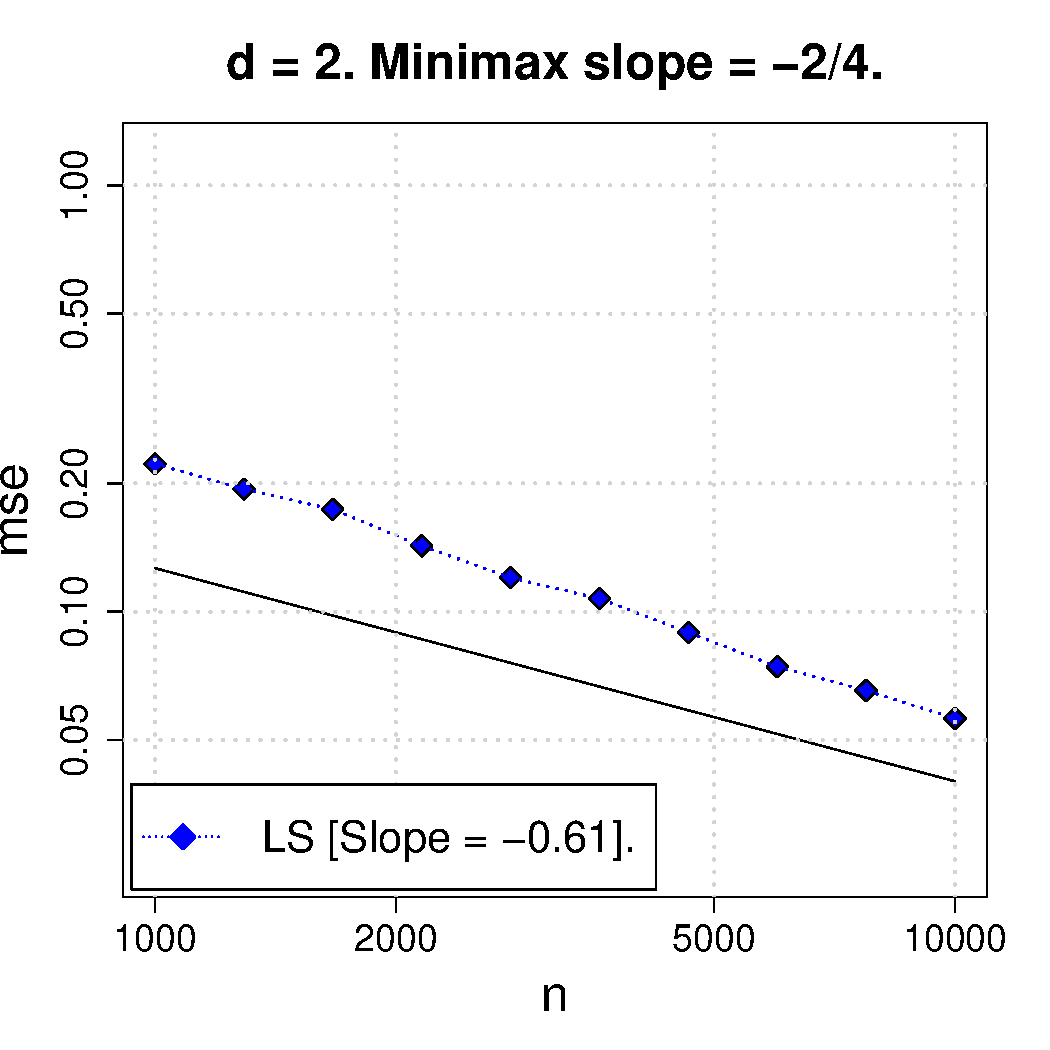
\includegraphics[width=.245\textwidth]{figures/cosine/mse_by_sample_size_2d.pdf}
	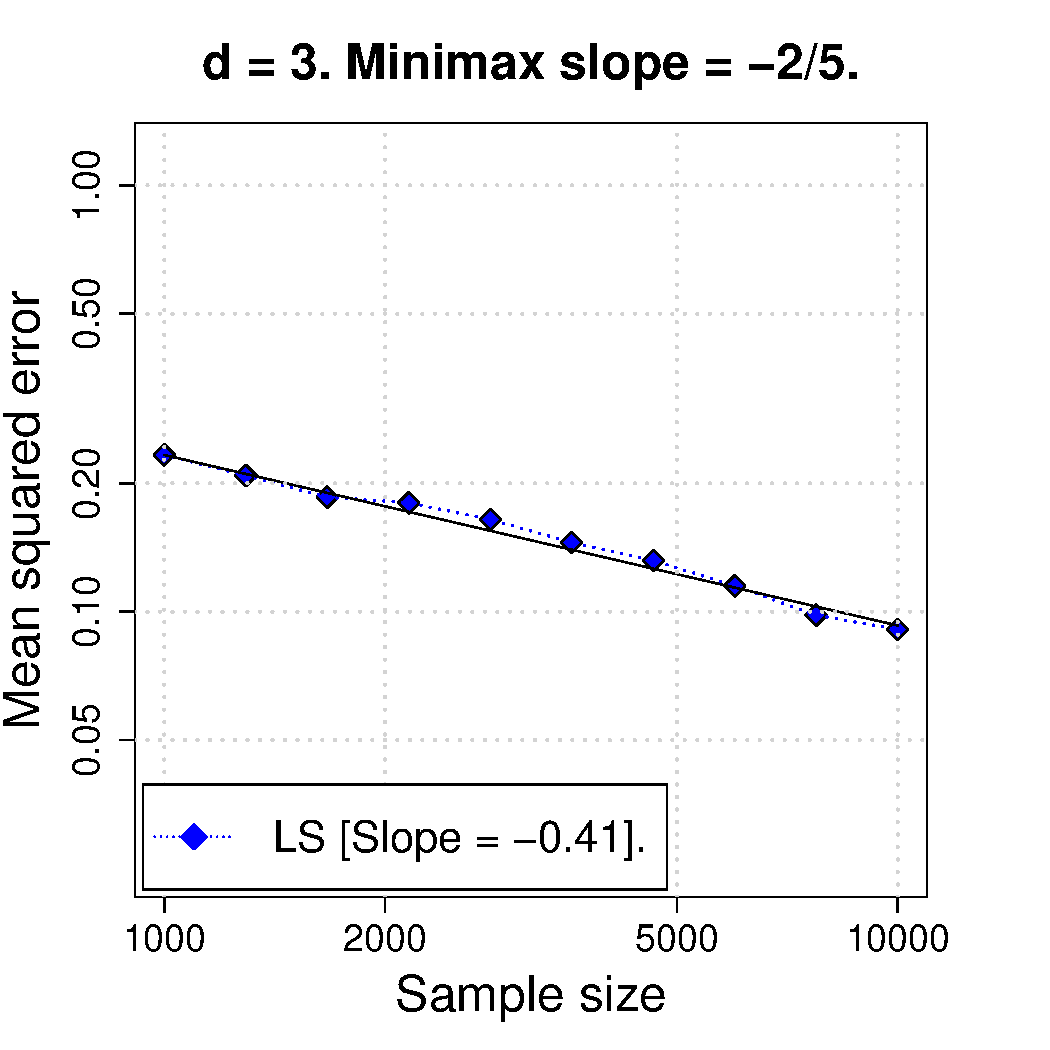
\includegraphics[width=.245\textwidth]{figures/cosine/mse_by_sample_size_3d.pdf} 
	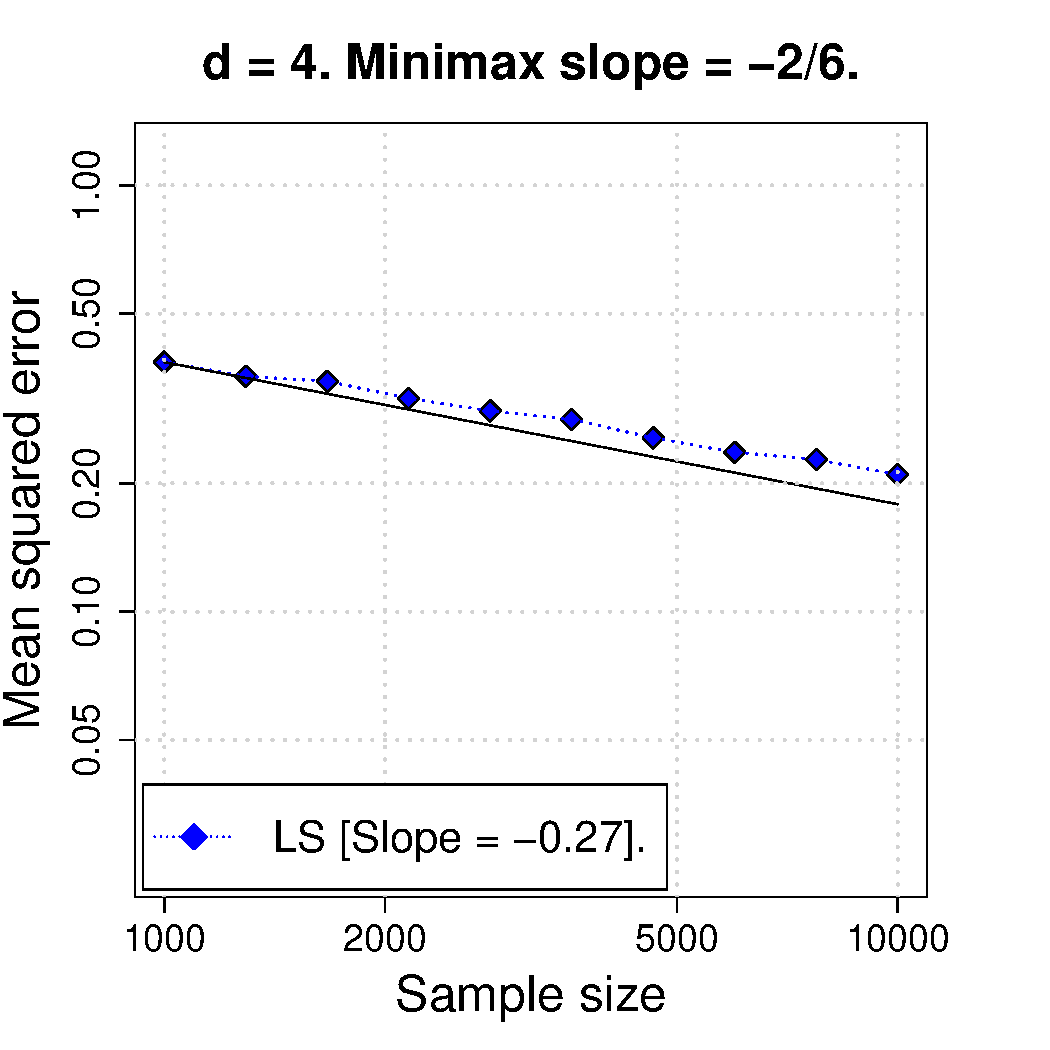
\includegraphics[width=.245\textwidth]{figures/cosine/mse_by_sample_size_4d.pdf}
	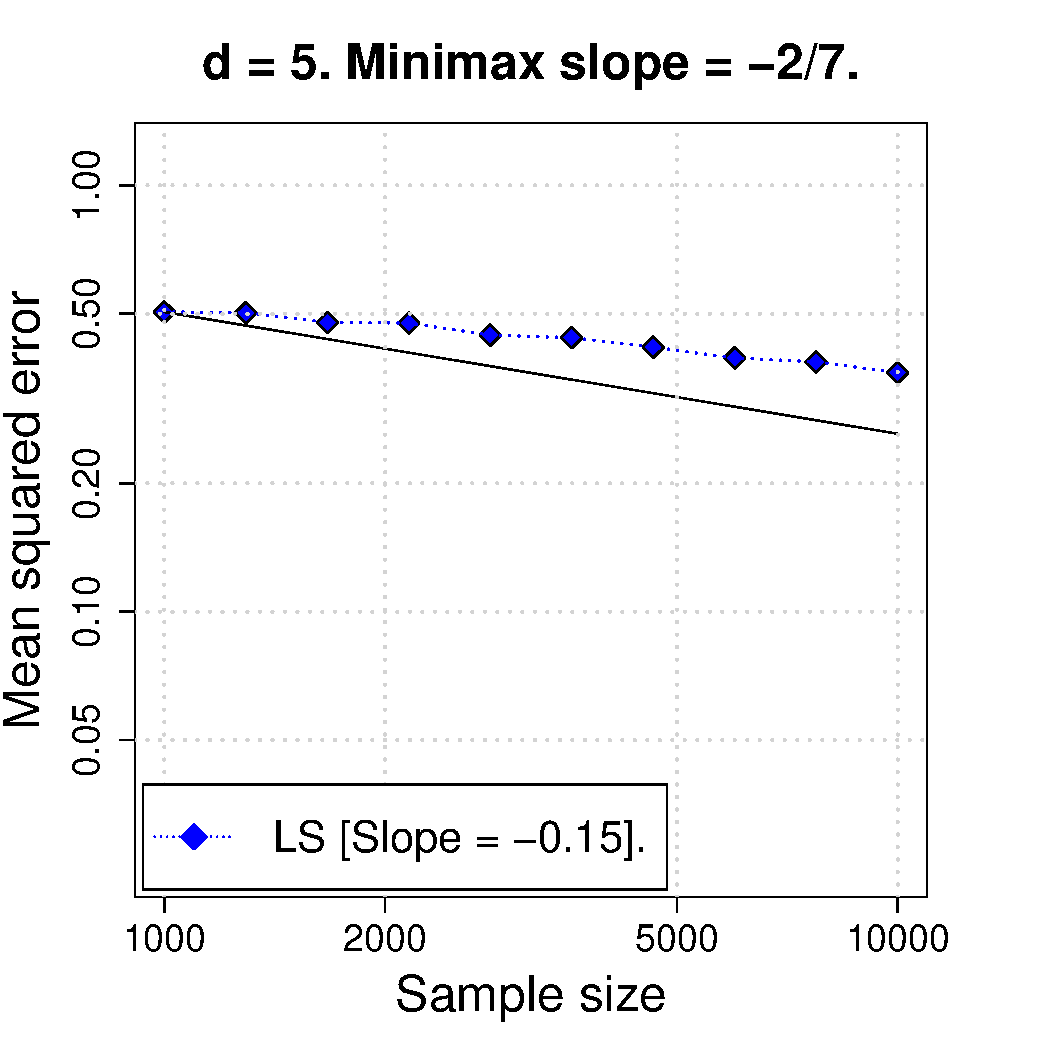
\includegraphics[width=.245\textwidth]{figures/cosine/mse_by_sample_size_5d.pdf}
	\caption{Mean squared error of Laplacian smoothing (\texttt{LS}) as a function of sample size $n$. Each plot is on the log-log scale, and the results are averaged over 5 repetitions, with Laplacian smoothing tuned for optimal average mean squared error. The black line shows the minimax rate (in slope only; the intercept is chosen to match the observed error).}
	\label{fig:fig1}
% RJT: Alden, please verify that what I wrote about the intercept above is right. And if so, can you redo the black line for d = 2 so that the intercept matches better? Thanks. Oh and if you're already going to redo one of these plots, you can satisfy my unreasonably nitpicky brain and change the x- and y-axes on all of them to use words rather than symbols/acronyms: "Sample size" and "Mean squared error". 
\end{figure*}

\paragraph{Testing Error of Laplacian Smoothing.}

For $b \geq 1$, define a threshold \smash{$\wh{t}_b$} as
\begin{equation*}
\wh{t}_{b} = \frac{1}{n}\sum_{k = 1}^{n} \frac{1}{(\rho \lambda_k + 1)^2} + \frac{2b}{n}\sqrt{\sum_{k = 1}^{n} \frac{1}{(\rho \lambda_k + 1)^4}},
\end{equation*}
where we recall $\lambda_k$ is the $k$th smallest eigenvalue of \smash{$\Lap_{n,r}$}. The Laplacian smoothing test is then simply
\begin{equation*}
\wh{\varphi} = \1\bigl\{\wh{T} \leq \wh{t}_b\bigr\}.
\end{equation*} 
%(Clearly \smash{$\wh{\varphi}$} depends on $b$, but we suppress this notationally.) 
Here $b \geq 1$ is a tuning parameter selected by the user, with the choice driven by the tolerated Type I versus Type II error. In fact, the threshold \smash{$\wh{t}_b$} is precisely the right choice to control the Type I error of \smash{$\wh{\varphi}$}: we show in the supplement that
\begin{equation}
\label{eqn:type_I_error}
\Ebb_0\bigl[\wh{\varphi}\bigr] \leq \frac{1}{b^2}.
\end{equation}
The next theorem shows that this test also has small Type II error, uniformly over all $f_0$ that are separated from $0$ by at least the critical radius given in \eqref{eqn:sobolev_space_testing_critical_radius}. For this to hold, we will require a tighter range of scalings for the radius $r$.
\begin{enumerate}[label=(R\arabic*)]
	\setcounter{enumi}{1}
	\item 
	\label{asmp:ls_kernel_radius_testing}
	For constants $C_0,c_0>0$, the neighborhood graph radius $r$ satisfies
	\begin{equation*}
	C_0\biggl(\frac{\log n}{n}\biggr)^{\frac{1}{d}} \leq r \leq c_0 \wedge M^{\frac{(d - 8)}{8 + 2d}} n^{\frac{d - 20}{32 + 8d}}.
	\end{equation*}
\end{enumerate}

Now define
\begin{equation*}
M_{\max}(d) =
\begin{cases*}
n^{1/8} & \textrm{$d = 1$} \\
n^{(4 - d)/(4d)} & \textrm{$d \geq 2$}.
\end{cases*}
\end{equation*}

Note that when $d < 4$ and $M \leq M_{\max}(d)$, there always exists a choice of $r$ which satisfies~\ref{asmp:ls_kernel_radius_testing}. 
We now state Theorem~\ref{thm:laplacian_smoothing_testing}, our main testing result.
\begin{theorem}
	\label{thm:laplacian_smoothing_testing}
  Given i.i.d.\ draws $(X_i,Y_i)$, $i=1,\ldots,n$ from \eqref{eqn:signal_plus_noise_model}, assume $f_0 \in H^1(\Xset,M)$ where $\Xset \subseteq \Rd$ with $d < 4$, and where $M \leq M_{\max}(d)$. Assume \ref{asmp:domain}, \ref{asmp:density} on the design distribution $P$, and assume \smash{$G_{n,r}$} is computed with a kernel $K$ satifsying \ref{asmp:kernel}. There are constants $N,C,c>0$ such that for any $n \geq N$, and any radius $r$ as in \ref{asmp:ls_kernel_radius_testing}, the Laplacian smoothing test \smash{$\wh{\varphi}$} based on the estimator \smash{$\wh{f}$} in \eqref{eqn:laplacian_smoothing}, with \smash{$L = L_{n,r}$} and \smash{$\rho = (nr^{d + 2})^{-1} n^{-4/(4 + d)} M^{-8/(4 + d)}$}, satisfies the following: for all $b \geq 1$, and all $f_0$ such that
	\begin{equation}
	\label{eqn:laplacian_smoothing_testing}
	\bigl\|f_0\bigr\|_{\Leb^2(\Xset)}^2 \geq C b^2 M^{2d/(4 + d)} n^{-4/(4 + d)},
	\end{equation} 
	the Type II error is upper bounded by
	\begin{multline*}
	\Ebb_{f_0}\bigl[1 - \wh{\varphi} \bigr] \leq \\
	C\biggl(\frac{1}{b}\Bigl[1 + n^{-d/(4 + d)}M^{-2d/(4 + d)}\Bigr] + n\exp\bigl(-cnr^d\bigr)\biggr).
	\end{multline*}
\end{theorem}

Some remarks:
\begin{itemize}
	\item As mentioned earlier, Sobolev balls $H^1(\Xset,M)$ for $d \geq 4$ include quite irregular functions $f \not\in \Leb^4(\Xset)$. Proving tight lower bounds in this case is nontrivial, and as far as we understand such an analysis remains outstanding. On the other hand, if we explicitly assume that $f_0 \in \Leb^4(\Xset,M)$, then \citet{guerre02} show that the testing problem is characterized by a dimension-free lower bound $\epsilon^{2}(\Leb^4(\Xset,M)) \gtrsim n^{-1/2}$. Moreover, by training \smash{$\wh{f}$} to the interpolation limit, setting $\rho = 0$, the subsequent test \smash{$\wh{\varphi}$} will achieve (up to constants) this lower bound. That is, for any $f_0 \in \Leb^4(\Xset,M)$ such that \smash{$\|f_0\|_{\Leb^2(\Xset)}^2 \geq C b^2n^{-1/2}$}, we have both
	\begin{equation}
	\label{eqn:laplacian_smoothing_testing_low_smoothness}
	\Ebb_{f_0}\bigl[1 - \wh{\varphi}\bigr] \leq \frac{C(1 + M^4)}{b^2},
	\end{equation} 
	and \smash{$\Ebb_0[\wh{\varphi}] \leq 1/b^2$}. Note that the same results apply to \smash{$\wt{T}$}, since the thin-plate spline estimator \smash{$\wt{f}$} interpolates the responses $Y_1,\ldots,Y_n$ for $d>1$.
	\item To compute the data-dependent threshold \smash{$\wh{t}_b$}, one must know all of the eigenvalues $\lambda_1,\ldots,\lambda_n$. Computing all these eigenvalues is far more expensive (cubic-time) than computing \smash{$\wh{T}$} in the first place (nearly-linear-time). But in practice we would not recommend using \smash{$\wh{t}_b$} anyway, and would instead we make the standard recommendation to calibrate via a permutation test \citep{hoeffding1952}. 
\end{itemize}

\paragraph{More Discussion of Variational Analog.}

With some results in hand, let us pause to offer some explanation of why Laplacian smoothing can be optimal in settings where thin-plate splines are not even consistent. First, we elaborate on why this difference in performance is so surprising. As mentioned previously, the penalties in \eqref{eqn:laplacian_smoothing}, \eqref{eqn:thin_plate_spline} can be closely tied together: \citet{bousquet03} show that for $f \in C^2(\Xset)$, 
\begin{equation}
\label{eqn:seminorm_consistency}
\begin{aligned}
\lim \frac{1}{n^2 r^{d + 2}} f^\top \Lap_{n,r} f & = \int_{\Xset} f(x) \cdot \Delta_Pf(x) p(x) \,dx \\
& = \int_{\Xset} \|\nabla f(x)\|_2^2 p^2(x) \,dx.
\end{aligned}
\end{equation}
In the above, the limit is as $n \to \infty$ and $r \to 0$, $\Delta_P$ is the (weighted) Laplace-Beltrami operator
\begin{equation*}
\Delta_Pf := -\frac{1}{p} \dive\bigl(p^2\nabla f),
\end{equation*}
and the second equality follows using integration by parts.\footnote{Assuming $f$ satisfies e.g., Dirichlet boundary conditions.} To be clear, this argument does not formally imply that $\wh{f}$ and $\wt{f}$ are close (for one, note that \eqref{eqn:seminorm_consistency} holds for $f \in C^2(\Xset)$, whereas the optimization in \eqref{eqn:thin_plate_spline} considers a much broader set of continuous functions with weak derivatives in $\Leb^2(\Xset)$). But it does seem to suggest that the two estimators should behave somewhat similarly. 

Of course, we know this is not the case: $\wh{f}$ and $\wt{f}$ look very differently when $d > 1$. What is driving this difference? The key point is that the discretization imposed by the graph $G_{n,r}$---which might seem problematic at first glance---turns out to be a blessing. The problem with~\eqref{eqn:thin_plate_spline} is that the class $H^1(\Xset)$, which fundamentally underlies the criterion, is far ``too big'' for $d > 1$. This is meant in various related senses. By the Sobolev embedding theorem, for $d>1$, the class $H^1(\Xset)$ does not continuously embed into any H\"{o}lder space; and in fact it does not even continuously embed into $C^0(\Xset)$. Thus we cannot really restrict the optimization to \emph{continuous} and weakly differentiable functions, as we could when $d=1$ (the smoothing spline case), without throwing out a substantial subset of functions in $H^1(\Xset)$. Even among continuous and differentiable functions $f$, as we explained previously, we can use ``bump'' functions (as in \citet{green93}) to construct $f$ that interpolates the pairs $(X_i,Y_i)$, $i=1,\ldots,n$ and achieves arbitrarily small penalty (and hence criterion) in \eqref{eqn:thin_plate_spline}. In this sense, any estimator resulting from solving \eqref{eqn:thin_plate_spline} estimator will clearly be inconsistent. 

On the other hand, problem \eqref{eqn:laplacian_smoothing} is finite-dimensional. As a result \smash{$\wh{f}$} has far less capacity to overfit than does \smash{$\wt{f}$}, for any given sample size $n$. Discretization is not the only way to make the problem \eqref{eqn:thin_plate_spline} more tractable: for instance, one can replace the penalty \smash{$\int_{\Xset} \|\nabla f(x)\|_2^2 \,dx$} with a stricter choice like \smash{$\esssup_{x \in \Xset} \|\nabla f(x)\|_2$}, or conduct the optimization over some finite-dimensional linear subspace of $H^1(\Xset)$ (i.e., use a sieve). While these solutions do improve the statistical properties of \smash{$\wt{f}$} for $d > 1$ (see e.g., \citet{birge1993,birge1998,vandergeer2000}), Laplacian smoothing is generally speaking much simpler and more computationally friendly, and in addition, the other approaches are specifically tailored to the domain $\Xset$, in stark to \smash{$\wh{f}$}.

\paragraph{Overview of Analysis.}

The comparison with thin-plate splines highlights some surprising differences between \smash{$\wh{f}$} and \smash{$\wt{f}$}. Such differences also preclude us from analyzing \smash{$\wh{f}$} by, say, using \eqref{eqn:seminorm_consistency} to establish a coupling between \smash{$\wh{f}$} and \smash{$\wt{f}$}---we know this cannot work, because we would like to prove meaningful error bounds on \smash{$\wh{f}$} in regimes where no such bounds exist for \smash{$\wt{f}$}.

Instead we take a different approach, and directly analyze the error of \smash{$\wh{f}$} and \smash{$\wh{T}$} using a bias-variance decomposition (conditional on $X_1,\ldots,X_n$). A standard calculation shows that
\begin{equation*}
\bigl\|\wh{f} - f_0\bigr\|_n^2 \leq \underbrace{\vphantom{\sum_{k=1}^n}\frac{2\rho}{n} \bigl(f_0^\top \Lap_{n,r} f_0\bigr)}_{\textrm{bias}} + \underbrace{\frac{10}{n} \sum_{k = 1}^{n} \frac{1}{(\rho \lambda_k + 1)^2}}_{\textrm{variance}},
\end{equation*}
and likewise that $\wh{\varphi}$ has high power whenever
\begin{equation*}
\bigl\|f_0\bigr\|_n^2 \geq \underbrace{\vphantom{\sqrt{\sum_{k=1}^n}}\frac{2\rho}{n} \bigl(f_0^\top \Lap_{n,r} f_0\bigr)}_{\textrm{bias}} + \underbrace{\frac{4b}{n} \sqrt{\sum_{k = 1}^{n} \frac{1}{(\rho \lambda_k + 1)^4}}}_{\textrm{variance}}.
\end{equation*}
The bias and variance terms are each functions of the random graph \smash{$G_{n,r}$}, and hence are themselves random. To upper bound them, we build on some recent works \citep{burago2014,trillos2019,calder2019} regarding the consistency of neighborhood graphs to establish the following lemmas. These lemmas assume \ref{asmp:domain}, \ref{asmp:density} on the design distribution $P$, and \ref{asmp:kernel} on the kernel used to compute the neighborhood graph \smash{$G_{n,r}$}. 

\begin{lemma}
	\label{lem:graph_sobolev_seminorm}
  There are constants $N,C_2 > 0$ such that for $n \geq N$, $r \leq c_0$, and $f \in H^1(\Xset)$, with probability at least $1 - \delta$, it holds that
	\begin{equation}
	\label{eqn:graph_sobolev_seminorm}
	f^\top \Lap_{n,r} f \leq \frac{C_2}{\delta} n^2 r^{d + 2} |f|_{H^1(\Xset)}^2.
	\end{equation}
\end{lemma}

\begin{lemma}
	\label{lem:neighborhood_eigenvalue} 
  There are constants $N,C_1,C_3,c_1,c_3 > 0$ such that for $n \geq N$, $C_0(\log n/n)^{1/d} \leq r \leq c_0$, and $f \in H^1(\Xset)$, with probability at least $1 - C_1n\exp(-c_1nr^d)$, it holds that
	\begin{equation}
	\label{eqn:neighborhood_eigenvalue}
	c_3A_{n,r}(k) \leq \lambda_k \leq C_3A_{n,r}(k), ~~\textrm{for $2 \leq k \leq n$},
	\end{equation}
where \smash{$A_{n,r}(k) = \min\{nr^{d + 2}k^{2/d},nr^d\}$}.
\end{lemma}

Lemma~\ref{lem:graph_sobolev_seminorm} gives a direct upper bound on the bias term. Lemma~\ref{lem:neighborhood_eigenvalue} leads to a sufficiently tight upper bound on the variance term whenever the radius $r$ is sufficiently small; precisely, when $r$ is upper bounded as in \ref{asmp:ls_kernel_radius_estimation} for estimation, or \ref{asmp:ls_kernel_radius_testing} for testing. The parameter $\rho$ is then tuned to minimize the sum of bias and variance, in the usual manner.

It may be useful to give one more perspective on our approach. A common strategy in analyzing penalized least squares estimators is to assume two properties: first, that the regression function $f_0$ lies in (or near) a ball defined by the penalty operator; second, that this ball is reasonably small, e.g., as measured by metric entropy, or Rademacher complexity, etc. In contrast, in Laplacian smoothing, the penalty induces a ball
\begin{equation*}
H^1(G_{n,r},M) := \{f: f^\top \Lap_{n,r} f \leq M^2\}
\end{equation*}
that is data-dependent and random, and so we do not have access to either of the aforementioned properties a priori, and instead, must prove they hold with high probability. In this sense, our analysis is different than the typical one in nonparametric regression.

\section{MANIFOLD ADAPTIVITY}
\label{sec:manifold_adaptivity}

The minimax rates $n^{-2/(2 + d)}$ and $n^{-4/(4 + d)}$, in estimation and testing, suffer from the curse of dimensionality. However, in practice it can be often reasonable to assume a \emph{manifold hypothesis}: that the data $X_1,\ldots,X_n$ lie on a manifold $\Xset$ of $\Rd$ that has intrinsic dimension $m < d$. Under such an assumption, it is known \citep{bickel2007,ariascastro2018} that the optimal rates over $H^1(\Xset)$ are now $n^{-2/(2 + m)}$ (for estimation) and $n^{-4/(4 + m)}$ (for testing), which are much faster than the full-dimensional error rates when $m \ll d$. 

% RJT: Again, would venture a guess that these are stated results for Holder classes, not Sobolev classes. So same comment as before, as when we referenced Tsybakov. Just checking my understanding ... not sure it's worth changing this at this point. 

On the other hand, a theory has been developed \citep{belkin03,belkin05,niyogi2013} establishing that the neighborhood graph $G_{n,r}$ can ``learn'' the manifold $\Xset$ in various senses, so long as $\Xset$ is locally linear. We contribute to this line of work by showing that under the manifold hypothesis, Laplacian smoothing achieves the sharper minimax rates over $H^1(\Xset)$.

\paragraph{Error Rates Assuming the Manifold Hypothesis.}

The conditions and results presented here will be largely similar to the previous ones, except with the ambient dimension $d$ replaced by the intrinsic dimension $m$. For the remainder, we assume the following.
\begin{enumerate}[label=(P\arabic*)]
	\setcounter{enumi}{2}
	\item 
	\label{asmp:domain_manifold}
	$P$ is supported on a compact, connected, smooth manifold $\Xset$ embedded in $\Rd$, of dimension $m \leq d$. The manifold is without boundary and has positive reach \citep{federer1959}.
	\item 
	\label{asmp:density_manifold} 
  $P$ admits a density $p$ with respect to the volume form of $\Xset$ such that 
	\begin{equation*}
	0 < p_{\min} \leq p(x) \leq p_{\max} < \infty, ~~\textrm{for all $x \in \Xset$}. 
	\end{equation*}
	Additionally, $p$ is Lipschitz on $\Xset$, with Lipschitz constant $L_p$.
\end{enumerate}

Under the assumptions \ref{asmp:domain_manifold}, \ref{asmp:density_manifold}, and \ref{asmp:kernel}, and for a suitable range of $r$, the error bounds on the estimator \smash{$\wh{f}$} and test \smash{$\wh{\varphi}$} will depend on $m$ instead of $d$. 
\begin{enumerate}[label=(R\arabic*)]
	\setcounter{enumi}{3}
	\item 
	\label{asmp:ls_kernel_radius_estimation_manifold}
	For constants $C_0,c_0>0$, the neighborhood graph radius $r$ satisfies 
	\begin{equation*}
	C_0\biggl(\frac{\log n}{n}\biggr)^{\frac{1}{m}} \leq r \leq c_0 \wedge  M^{\frac{(m - 4)}{(4 + 2m)}} n^{\frac{-3}{(4 + 2m)}}.
	\end{equation*}
\end{enumerate}

\begin{theorem}
	\label{thm:laplacian_smoothing_estimation_manifold}
  As in Theorem \ref{thm:laplacian_smoothing_estimation1}, but where $\Xset \subseteq \Rd$ is now a manifold with intrinsic dimension $m < 4$, and the design distribution $P$ obeys \ref{asmp:domain_manifold}, \ref{asmp:density_manifold}. There are constants $N,C,C_1,c,c_1>0$ (not depending on $f_0$) such that for any $n \geq N$, and any radius $r$ as in \ref{asmp:ls_kernel_radius_estimation_manifold}, the Laplacian smoothing estimator \smash{$\wh{f}$} in \eqref{eqn:laplacian_smoothing}, with \smash{$L = L_{n,r}$} and \smash{$\rho = M^{-4/(2 + m)} (nr^{m + 2})^{-1} n^{-2/(2 + m)}$}, satisfies
	\begin{equation*}
	\bigl\|\wh{f} - f_0\bigr\|_n^2 \leq \frac{C}{\delta} M^{2m/(2 + m)} n^{-2/(2 + m)},
	\end{equation*}
  with probability at least $1 - \delta -  C_1 n\exp(-cnr^m) - \exp(-c \min\{M^{m/(2m + 4)} n^{m/(2+m)},n\})$.
% RJT: Alden, please verify that what I wrote is correct.
\end{theorem}

\begin{enumerate}[label=(R\arabic*)]
	\setcounter{enumi}{4}
	\item 
	\label{asmp:ls_kernel_radius_testing_manifold}
	For constants $C_0,c_0>0$, the neighborhood graph radius $r$ satisfies 
	\begin{equation*}
	C_0\biggl(\frac{\log n}{n}\biggr)^{\frac{1}{m}} \leq r \leq c_0 \wedge M^{\frac{(m - 8)}{8 + 2m}} n^{\frac{m - 20}{32 + 8m}}.
	\end{equation*}
\end{enumerate}

\begin{theorem}
	\label{thm:laplacian_smoothing_testing_manifold}
  As in Theorem \ref{thm:laplacian_smoothing_testing}, but where $\Xset \subseteq \Rd$ is a manifold with intrinsic dimension $m < 4$, $M \leq M_{\max}(m)$, and the design distribution $P$ obeys \ref{asmp:domain_manifold}, \ref{asmp:density_manifold}.
There are constants $N,C,c>0$ such that for any $n \geq N$, and any $r$ as in \ref{asmp:ls_kernel_radius_testing_manifold}, the Laplacian smoothing test \smash{$\wh{\varphi}$} based on the estimator \smash{$\wh{f}$} in \eqref{eqn:laplacian_smoothing}, with \smash{$L = L_{n,r}$} and \smash{$\rho = (nr^{m + 2})^{-1} n^{-4/(4 + m)} M^{-8/(4 + m)}$}, satisfies the following: for all $b \geq 1$, and $f_0$ such that
	\begin{equation}
	\label{eqn:laplacian_smoothing_testing_manifold}
	\bigl\|f_0\bigr\|_{\Leb^2(\Xset)}^2 \geq C b^2 M^{2m/(4 + m)} n^{-4/(4 + m)},
	\end{equation} 
	the Type II error is upper bounded by
	\begin{multline*}
	\Ebb_{f_0}\bigl[1 - \wh{\varphi} \bigr] \leq \\
	C\biggl(\frac{1}{b}\Bigl[1 + n^{-m/(4 + m)}M^{-2m/(4 + m)}\Bigr] + n\exp\bigl(-cnr^m\bigr)\biggr).
	\end{multline*}
% RJT: Alden, please verify that what I wrote is correct.
\end{theorem}

The proof of Theorems \ref{thm:laplacian_smoothing_estimation_manifold} and \ref{thm:laplacian_smoothing_testing_manifold} proceeds in a similar manner to that of Theorems \ref{thm:laplacian_smoothing_estimation1} and \ref{thm:laplacian_smoothing_testing}. The key difference is that in the manifold setting, the equations \eqref{eqn:graph_sobolev_seminorm} and \eqref{eqn:neighborhood_eigenvalue} used to upper bound bias and variance will hold with $d$ replaced by $m$.

We emphasize that little about $\Xset$ needs be known for Theorems~\ref{thm:laplacian_smoothing_estimation_manifold} and \ref{thm:laplacian_smoothing_testing_manifold} to hold. Indeed, all that is needed is the intrinsic dimension $m$, to properly tune $r$ and $\rho$ (from a theoretical point of view), and otherwise \smash{$\wh{f}$} and \smash{$\wh{\varphi}$} are computed without regard to $\Xset$. In contrast, the penalty in \eqref{eqn:thin_plate_spline} would have to be specially tailored to work in this setting, revealing another advantage of the discrete approach to the variational one.

\section{DISCUSSION}
\label{sec:discussion}

We have shown that Laplacian smoothing, computed over a neighborhood graph, can be optimal for both estimation and goodness-of-fit testing over Sobolev spaces. There are many extensions worth pursuing, and several have already been mentioned. We conclude by mentioning a couple more. In practice, it is more common to use $k$-nearest-neighbor (kNN) graphs than neighborhood graphs, due to the guaranteed connectivity and sparsity of the former; we suspect that by building on the work of \citet{calder2019}, one can show that our main results all hold under the kNN graph as well. In another direction, one can also generalize Laplacian smoothing by replacing the penalty \smash{$f^\top \Lap_{n,r} f$} with \smash{$f^\top \Lap_{n,r}^k f$} for $k > 1$. The hope is that this would then achieve minimax optimal rates over the higher-order Sobolev class $H^k(\Xset)$. % In the very special case of $k = 2$ and $d \leq 2$, we can show that this is indeed the case, but the general story--for all combinations of $k$ and $d$---remains beyond our reach. 

\bibliographystyle{plainnat}
\bibliography{../../../graph_regression_bibliography} 

\end{document}